\documentclass[journal]{./IEEE/IEEEtran}
\usepackage{cite,graphicx}
\usepackage{graphicx}
\usepackage{xcolor}
\usepackage{xurl}
\usepackage{hyperref}
\usepackage{blindtext}

\usepackage[justification=centering, font=footnotesize]{caption}
\captionsetup{justification=raggedright,singlelinecheck=false}


\newcommand{\SPTITLE}{Scheduling of Patrols Within the UPLB Campus Using an Opportunistic Crime Security Game}
\newcommand{\ADVISEE}{Karl Jasson B. Pios}
\newcommand{\ADVISER}{Jaderick P. Pabico}

\newcommand{\BSCS}{Bachelor of Science in Computer Science}
\newcommand{\ICS}{Institute of Computer Science}
\newcommand{\UPLB}{University of the Philippines Los Ba\~{n}os}
\newcommand{\REMARK}{\thanks{Presented to the Faculty of the \ICS, \UPLB\
                             in partial fulfillment of the requirements
                             for the Degree of \BSCS}}
        
\markboth{CMSC 190 Special Problem, \ICS}{}
\title{\SPTITLE}
\author{\ADVISEE~and~\ADVISER%
\REMARK
}
\pubid{\copyright~2022~ICS \UPLB}

%%%%%%%%%%%%%%%%%%%%%%%%%%%%%%%%%%%%%%%%%%%%%%%%%%%%%%%%%%%%%%%%%%%%%%%%%%

\begin{document}

% TITLE
\maketitle

% ABSTRACT
\begin{abstract}
%The abstract should be \textit{inffreedom park andormational}. Typically a single paragraph
%of about fifty to two hundred workds, the abstract allows your readers to judge
%whether or not the article is of relevance to them. It should therefore be
%a concise summary of the aims, scope, and conclusions of your work. There
%is no space for unnecessary texts; an abstract should be kept to as few words
%as possible while remaining reasonably informative. Irrelevancies, such as
%minor details or a \textit{description} of the structure of the paper, are 
%inappropriate, as are acronyms, abbreviations, and mathematics. Sentences such
%as ``we review relevant literature" should be omitted.\cite{Zobel97}

UPLB's security firm, the University Police Force, is tasked with protecting property and ensuring safety of the public inside campus. Patrols are deployed within campus in an effort to maintain order and deter crime, but traditional methods are prone to inefficiency and predictability. This study aims to utilize game theory as an aid in deploying patrol units. Patrols movement must be effective without creating predictable patterns. With the use of weighted probabilities, randomization, and historical data, the UPF will be capable of scheduling optimal patrols with limited resources, while avoiding predictability at the same time. Historical data will be used to determine which areas of the campus have higher priority for patrolling. The system must also be able to deploy the patrols such that adversaries find it hard to predict their next move. Upon deploying patrols to areas, the scheduling program must take into account the distance that each patrol has travelled. This scheduling approach is seen to be more efficient and robust in scheduling patrols than other traditional methods, such as pure randomization. The scheduling system is capable of maximizing patrol coverage amidst the limitations on personnel numbers, and remain resilient against predictability.

\end{abstract}

% INDEX TERMS

\begin{keywords}
opportunistic crime, game theory, security game
\end{keywords}

% INTRODUCTION
\section{Introduction}
%To be effective, the introduction should answer the questions ``Why and What For (Four)?" Expanded, these questions are:\cite{Papadakis83}

\subsection{Background of the Study}
%Paragraph about security and how patrolling remains as a very enduring method
Security is a continuous concern worldwide. For every individual, it is important to protect their lives and their properties. Law enforcement and private security firms are tasked with protecting the general public from potential harm. These agencies need to establish effective campaigns in order for the public to go about their day with a good sense of security. Patrolling still remains as one of the most utilized campaigns implemented across the world. Effective patrolling is fundamental for maintaining stakeholders' trust.

%Patrols are deployed in ports, airports, and transport terminals in order to protect them from terrorist attacks. Private patrols have been employed to protect endangered wildlife and forests against poachers, illegal loggers, and the like. In public communities, law enforcement patrols move around to prevent crime, enforce laws, respond to distress calls, and maintain order. Security patrols are fundamental for keeping public trust and safety.

There are two primary problems faced by agencies when it comes to deploying patrols: limitations to resources, and the challenge of avoiding predictability. 

First, agencies have to perform tasks with limited resources. The ideal scenario is to deploy patrols in every area of their jurisdiction to maximize visibility and attack deterrence, but this comes at a very high cost, and agencies may not have the sufficient resources to achieve full coverage. With a finite amount of patrols, agencies have to deploy them strategically to maximize effectiveness.

Second, agencies have to contend with the fact that their movements are potentially monitored. As patrols are deployed over time, criminals, attackers, and other potential adversaries can observe their movements. If a routine or a pattern is found, adversaries can easily predict patrol movements and exploit vulnerabilities. Agencies have to take this into account, making sure that no patterns appear as they deploy patrols. They need to regularly variate the patrol schedules and routes in order to throw the adversaries off.

The challenge for security agencies is to deploy a finite number of patrols such that they maximize the effectiveness of their movements and avoid predictability at the same time. Implementing randomization may help in avoiding predictability. Full randomization, however, could cause inconsistencies, lacking assurance that each area will be patrolled sufficiently. Deployment may become inefficient, and multiple areas may be left vulnerable. The solution is to utilize randomization that set weighted probabilities for high and low risk areas. In this way, higher priority areas are guaranteed a good share of visits, while lower priority areas will not be neglected entirely.

Over the years, researchers have developed and implemented systems that aid agencies in deploying patrols effectively while avoiding predictability. These systems are capable of maintaining randomness without the personal biases that a human scheduler would be susceptible to. These systems have been used for airport terminals, air marshal deployment, protection of endangered wildlife and protected forests, and patrols along public transport systems.

\subsection{Statement of the Problem}
The University Police Force (UPF) is the official security division of the University of the Philippines Los Ba\~{n}nos (UPLB). Coordinating with community volunteers and a private security agency, UPF is tasked with protecting infrastructure, resources, and people from harm. The UPLB campus is open to the public; visitors and locals mix in with students and staff in the campus's public spaces. Guards at the access points cannot conduct thorough inspections due to the volume of people going in and out the campus.

In an effort to prevent crimes and policy violations from occurring within campus premises, as well as provide aid in sudden incidents, personnel are deployed to conduct patrols, done on foot or with a vehicle. They are deployed in specified zones within campus, and throughout their shift, patrols randomly move, on their own free will, from place to place within their zones. \\\\

The UPF, however, implements their methods without assistance from a system, making their patrols susceptible to inefficiency and ineffectiveness.

The lack of explicit route orders causes difficulties in monitoring and regulating patrols. It becomes difficult for UPF to guarantee that high priority areas are patrolled sufficiently, and some secluded areas may be left unguarded for too long. The patrols themselves are also susceptible to their personal biases. Randomizing their movement becomes harder over time, increasing the tendency to develop predictable movement patterns.

This study proposes a system that will assist the UPF in scheduling their patrols. The  system's main scheduling algorithm will assist in deploying their patrols, keeping visit frequencies consistent and avoiding predictability at the same time. Deployed patrols are expected to be able to follow route orders and accommodate emergency responses easily. Historical data will be used to identify high priority areas, and dynamic factors, such as, time of day, and civilian movement will be parameters for the system as well. An agent-based model will be used to visualize and simulate patrol movement within campus.

\subsection{Significance of the Study}

The developed scheduling program will assist UPF in optimally deploying patrols throughout the campus. High priority areas will be visited sufficiently and consistently, erasing possible irregular frequencies caused by purely randomized movement. Predictability is still avoided as the system ensures that no movement patterns will emerge. The patrols will be more effective in deterring adversaries from carrying out their intentions. This would allow UPF to be more effective in keeping campus premises protected without increasing operational cost.

\subsection{Objectives}
The primary objective of the study is to develop and implement a system that strategically schedules a finite number of patrols within the premises of the UPLB campus to prevent adversaries from finding opportunities to attack. Specifically:
\begin{enumerate}
\item{to develop a scheduler that creates an optimal strategy given limited patrol resources}
\item{to implement patrol strategies and random selection to limit the predictability of patrol movements and reduce crime opportunities}
\item{to utilize historical data in adjusting parameters and subsequent strategies}
\end{enumerate}

\section{Review of Related Literature}

Game theory is defined as the study of strategic interactions between rational individuals. Rationality implies that each individual is aware of what actions they can take and how their preferred actions can affect the outcome. Game theory aims to model strategic behaviour mathematically, particularly in interactions with conflict of interest.\cite{kockesen2007introduction} Studies in economics were the main motivation for developments in game theory, but over time applications have emerged in biology, computer science, social science, and engineering as well.

In the normal form of a game, players make their moves simultaneously. In a Stackelberg game, one player, called the ``leader'', makes their move first. The other players, called ``followers", see the move the leader picked and makes their own moves to maximize their benefit. The Stackelberg model heavily resembles the interaction between a security firm and their enemies.\cite{kar2017trends}

In a Stackelberg Security Game, the defender(leader) must protect potential targets with a finite amount of resources, knowing that attackers(followers) are observing their movement and planning an attack.\cite{kar2017trends} The defender implements one of multiple pure strategies for deployment, but the selection is done with randomization, making it a mixed strategy. Implementing mixed strategies prevent attackers from predicting the movements of the defender.\cite{an2017stackelberg}

There are three distinct categories of SSGs: infrastructure security games, \textit{green security} games, and opportunistic crime security games.\cite{an2017stackelberg} Infrastructure security games protect airports, terminals and other similar infrastructure that could be targeted by terrorism and organized crime.\cite{krausarmor} These attackers take long periods observing the area and the security detail, and they make careful plans of their operation. Infrastructure security games are considered "one-shot games". The defender will repeatedly deploy their strategy over weeks or months, but it only takes one successful attack to end the game.\cite{an2017stackelberg}

\textit{Green security} games involve protecting wildlife and the natural environment from poachers, illegal loggers, people using illegal fishing methods, etc.\cite{fang2017paws} The main characteristic of these games is that patrols have to adjust to the target's movements. Animals move around their habitat often, and forests may sprawl or shrink drastically. Attackers here do not need as much care in planning as terrorists do. These games are repeated games, as attackers commit multiple attacks. Successful attacks do not automatically end the game. Instead, the defender updates the strategies based on the obtained data from the previous attacks, and the cycle repeats itself.\cite{an2017stackelberg}

Opportunistic crime security games (OCSGs) protect the general public and their properties from acts of crime, such as theft and robbery.\cite{zhang2016opportunistic} Opportunistic criminals may have limitations in observing defender moves, but they are more flexible, easily moving to the next target if security deters them.\cite{zhang2016keeping} OCSGs are not explicitly formulated as repeated games. The defenders deploy their strategy, aiming to deter as many attacks as possible until the next strategy change. Crime reports and historical data are used to update strategies.\cite{an2017stackelberg}

Opportunity plays a significant role in urban crime. Crime needs three elements to occur: a vulnerable target, a likely offender, and the absence of a capable guardian.\cite{felson1998opportunity} OCSGs aim to deter crime by minimizing opportunity. Randomized patrols make it harder for criminals to determine when and where they can attack.\cite{paruchuri2007keep} When criminals perceive that finding opportunities is too costly, or the risk involved is too high, they can be deterred.\cite{felson1998opportunity}

There are three primary challenges to developing SSGs. The first challenge is \textit{scalability}. As the number of targets, activities, or resources increase, the strategy space expands exponentially. Systems would take longer to genrate strategies, and it would be more difficult to verify the quality of the output.\cite{tsai2009iris} Upscaling the security domain would require adjustments in the system to allow it to handle the increased complexity.\cite{pita2011guards}  

The second challenge is \textit{robustness}. Assumptions may be inaccurate in the real world, which meant that there are numerous uncertainties the algorithm must be able to handle.\cite{yin2013addressing} Patrols may encounter interruptions that the system cannot take into account, causing schedule disruptions. There are also uncertainties in the attackers, since they are also susceptible to doing sub-optimal decisions.\cite{pita2009effective}  

The third challenge is \textit{bounded rationality}. Most games assume that participants are rational and select the optimal decision. In the real world, human beings are not perfectly rational.\cite{abbasi2015human} Attackers in OCSGs deviate from the optimal strategy more than attackers in infrastructure or green security games. This can be attributed to the attackers lacking complete information, but it can also be linked to other factors such as past attempts or personal biases.\cite{sinha1human}

Traditional computer science approaches of evaluation, such as runtime analysis, would be irrelevant for SSGs. There are mathematical, qualitative, quantitative, and behavioural approaches for evaluation. Simulations, mock attacks, Expert analysis and human psychological studies are among the solutions present, and each approach vary in accuracy and cost.\cite{taylor2010framework}

% MATERIALS AND METHODS
\section{Materials and Methods}
The scheduler was developed in a machine with Windows 8.1 operating system. The scheduling software was developed with the following:

\begin{itemize}
\item{Java version 11} 
\item{Eclipse IDE version 2020-12}
\end{itemize}


\subsection{Zone Division}

The scheduling program will divide the UPLB campus into three distinct \textit{zones}. These divisions are based on geographical and environmental constraints of the campus. Each zone is further divided into \textit{patches}, and patrols can freely move within the patch they're assigned to. The user sets how many patrols are placed in each zone. The system guarantees that the patrol will not be assigned to visit patches outside of the zone it's assigned to.

%The first zone covers the section of the lower campus situated north of Molawin Creek, which includes the areas surrounding Carabao Park, Oblation Park, Main Library, and the Math Building. This zone is divided into eight patches. The second zone is the other section of the lower campus south of the creek. This zone covers the Freedom Park and the surrounding buildings, as well as parts of the College of Engineering and Agro-Industrial Technology (CEAT) and College of Veterinary Medicine (CVM).

The first zone covers the section of the lower campus situated north of Molawin Creek, which includes the areas surrounding Carabao Park, Oblation Park, Main Library, and the Math Building. The second zone is the other section of the lower campus south of the creek. This zone covers the Freedom Park and its vicinity, as well as parts of the College of Engineering and Agro-Industrial Technology (CEAT) and College of Veterinary Medicine (CVM). The third zone covers the Forestry Campus. The three zones are divided into eight, six, and four \textit{patches}, respectively. Figure 1 shows the zone divisions and their patches. 

\begin{figure}[h]
\centering
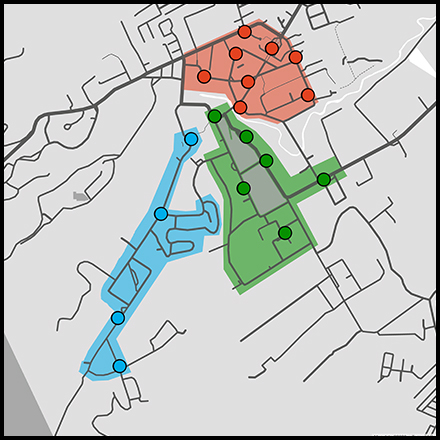
\includegraphics[scale=0.40]{./Images/campuszones_uplb.jpg}
\caption{The campus is divided into three zones, highlighted using three different colors.}
\end{figure}

The campus division was done this way due to several factors affecting each zone. The first zone has the most patches because of the density of buildings in the area. For a patrol standing at any point within the zone, their line of sight is frequently obstructed by buildings. When each patrol has decreased field of vision, vantage points have smaller coverage areas, thus the need to increase the number of patches. The second zone has a larger land area, but the zone mostly is very open space, particularly in the areas surrounding Freedom Park. In the third zone, most key areas are compactly placed along the main road, thus each patrol can easily cover a significant area of interest.

Dividing the campus into zones have several benefits. Keeping a patrol within its assigned zone allows the algorithm to calculate the next assignment faster, as it only needs to account for a section of the campus. The division also prevents the scheduler from clumping all the patrols in a small area of the map.

The zoning method only prevent patrols from being assigned to distant patches. In the real world, it does not restrict patrols from moving in between zones. This is important for interruptions, such as an emergency call to action. With the zoning limitations ensuring that patrols are spread across campus, the average response time would be minimized.

\subsection{Weighted Probability}
%weight intro
Each patch is given a \textit{weight} value. The said value determines the probability of the patch being selected by the scheduling algorithm. For handling this task, the developers decide to use the Java class \textit{EnumeratedDistribution}. Upon initialization, the EnumeratedDistribution class takes a \textit{List} of \textit{Pairs} as a parameter. Each Pair is comprised of an \textit{Object} class and its weight, stored as a \textit{Double} class. The probability distribution is based on the sum of all the weight values in the list. see figure

Using this method yields several advantages. If any of the weight values are adjusted, the EnumeratedDistribution class can implicitly handle the changes to the probability distribution. Sampling multiple items from the list is also possible, in which the developer only has to update the list after every sampling. This would be useful when selecting multiple patches from the set.

With the program dividing the campus into three zones, changing the weight value of a patch only affects the probability of the zone that patch belongs to. This means that each zone has a probability distribution that is independent from the others. Historical data can be utilized to adjust the probabilities and make them more representative of the real world problem.

%\begin{figure}[h]
%\begin{center}
%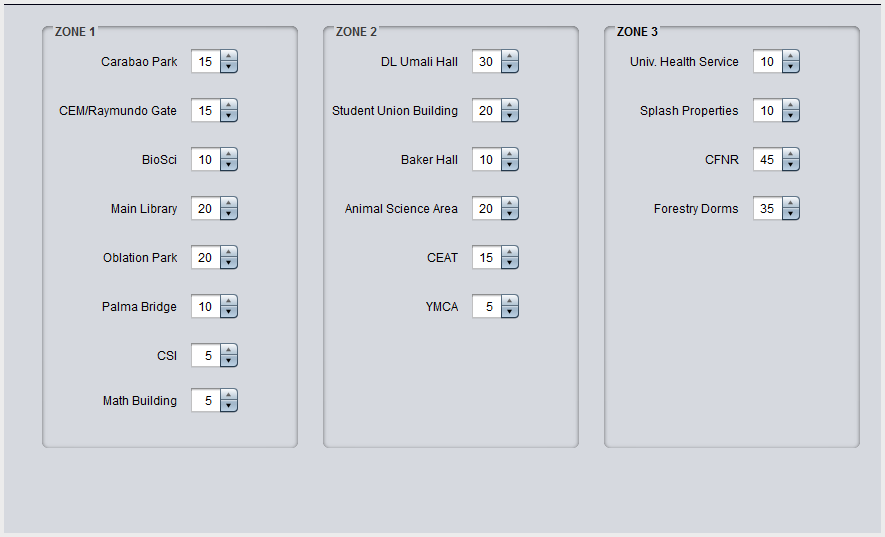
\includegraphics[scale=0.45]{./Images/weightsPanel.png}
%\caption{sample list of Patch and Weight values for sampling}
%\end{center}
%\end{figure}

\subsection{Scheduling Procedure}
The scheduling program first asks the user for the following inputs:

\begin{enumerate}
\item{Number of patrols allocated per zone}
\item{Number of intervals to be generated}
\item{Length of each interval (10, 15, 20, 30, or 60 minutes)}
\end{enumerate}

The second and third inputs determine how long the generated schedule would be. It is recommended that the schedule length do not exceed eight hours, which is the prescribed length for personnel duty. Changes made to these three parameters would cause a reset to the scheduler, and any generated schedules at that point will be erased. Figure 2 below shows a snippet of the scheduler's interface where the end user inputs the parameters.

\begin{figure}[h]
\centering
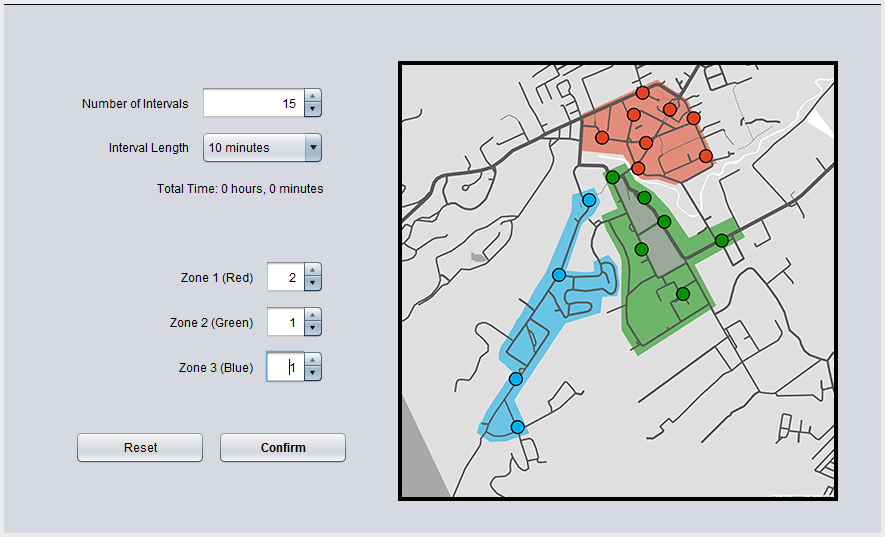
\includegraphics[scale=0.3]{./Images/parametersPanel.png}
\caption{The program asks the user for the key parameters to be used in the scheduling algorithm.}
\end{figure}

When the initial parameters are set, the next panel will show the user the weight values of the patches. The interface shows three sections for the three zones. These values have a default preset, set in place by the developer. The program is able to save multiple presets, and users can change values of an existing preset or create a new one. Figure 3 shows the program interface where the end user can change the weight values of each patch.

\begin{figure}[h]
\centering
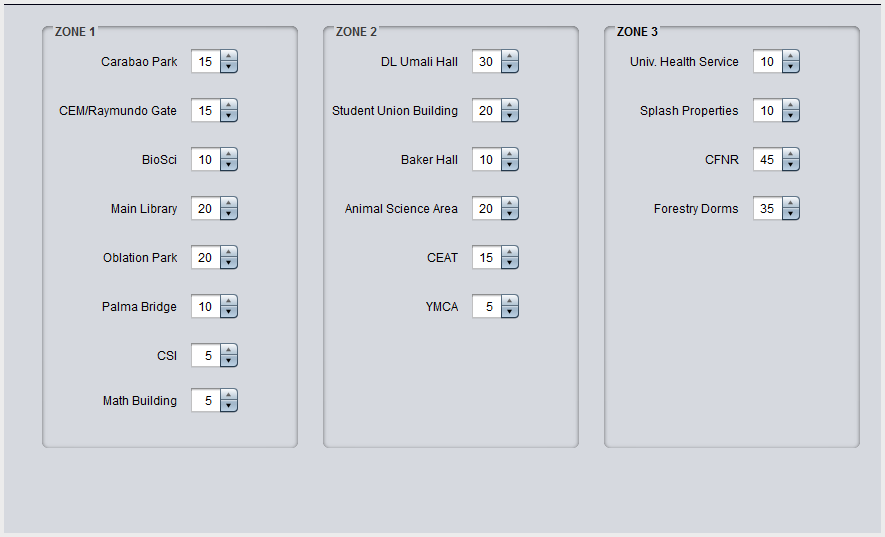
\includegraphics[scale=0.3]{./Images/weightsPanel.png}
\caption{The program allows adjustments to the probability of each patch.}
\end{figure}

When the patrol allocations and the patch weights are set, the scheduler proceeds through scheduling. For every interval, patches are selected in each zone equivalent to the number of allocated patrols. For cases where the number of patrols in a zone exceed the number of patches available, in which case the scheduler simply moves on to the next zone.

The generated schedule can be presented in text form (Figure 4) or graphical form (Figure 5). The graphical form, as seen in Figure 4, allows the end user to quickly inspect if there are patches that are either overprotected or vulnerable for too long, and assess the schedule and the probability distributions.

\begin{figure}[h]
\centering
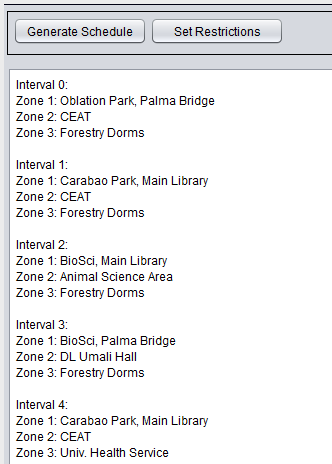
\includegraphics[scale=0.5]{./Images/schedulePanel.png}
\caption{A sample generated schedule, presented in text form.}
\end{figure}

\begin{figure}[h]
\centering
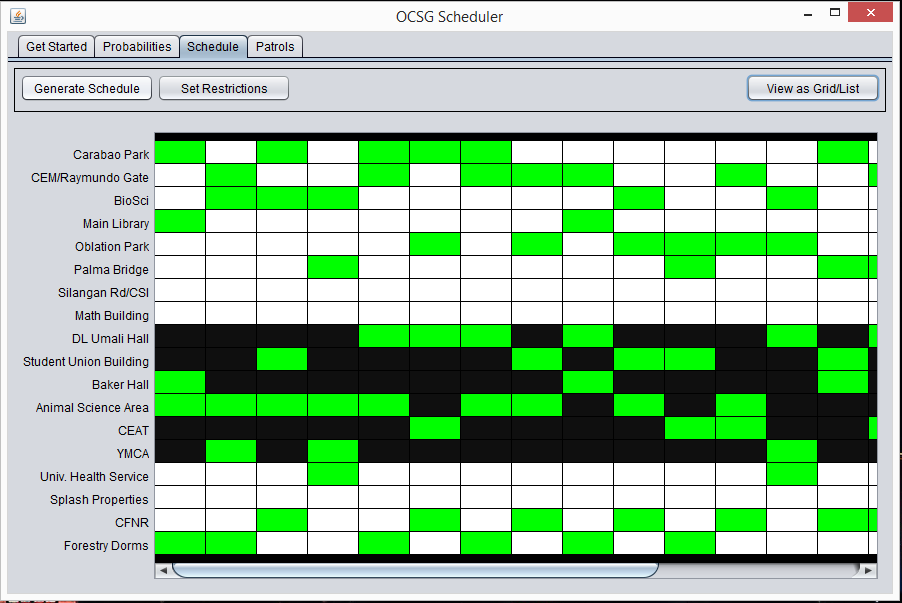
\includegraphics[scale=0.3]{./Images/ScheduleVisuals.png}
\caption{A schedule presented graphically. Consecutive green boxes mean a patch is guarded across several intervals.}
\end{figure}

At this point the user is then allowed to make several actions. The program can generate a new schedule using the same distributions. The user can also make adjustments to the probability distribution before generating a new schedule. Schedules will vary with timing, but the frequency of visits each patch is expected to be fairly consistent.



%The user is also allowed to set restrictions for a specific interval. A restriction can force the scheduler to explicitly select a patch, or ignore a patch. The restrictions are followed even if the user opted to redo schedule creation, but can also be removed.

\subsection{Assignment of Patrols}
At this point, the program only selected which patches in campus are to be patrolled. It did not assign which patrol unit will go to what patch. Assigning patrols to the selected patches should take into account each patrol's \textit{mileage}, or the total distance they have travelled. Patrols will not be assigned to areas that are too far from their current location throughout the duration of the schedule.

Since patch selection is based on probability and not proximity, there will be instances that a unit must travel a significant distance from its current location to the patch it is assigned to. The scheduling program must keep the mileages of the patrols in a zone to be as close to each other as possible. However, if there is only a single patrol in each zone, the mileage is fully dependent on the selected patches and their order.

There is no reliable method to determine the exact coordinates of each patrol since they are free to roam around the patch. To calculate from one patch to every other patch within the zone, each patch has a reference point that is used for calculating the distance. This values will be used to add to the mileage of each patrol, as they travel between patches. Due to this the mileage values of the patrols may not be equal to the actual mileage accumulated in the real world.

When the program assigns a patrol to the patch, it deploys the patrol with the highest mileage to the patch nearest to that patrol. This method keeps the averages lower. This also makes sure that no patrol is staying in one place too often. This is useful in certain schedules where a high probability patch is selected for consecutive intervals, patrols will still be rotated so they don't overstay. Figure 6 shows a sample of the scheduler displaying the patrol units, their assigned zone (indicated by color), and their mileages.

\begin{figure}[h]
\begin{center}
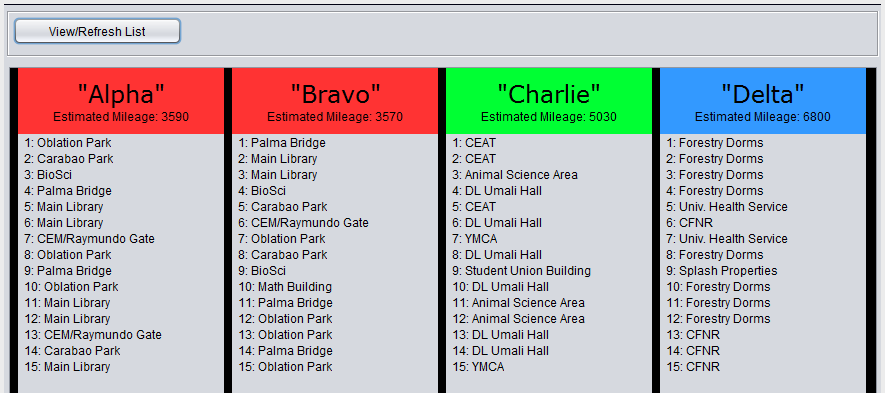
\includegraphics[scale=0.35]{./Images/patrolsPanel.png}
\caption{A program snippet that show each patrol's assignment over 15 intervals. The two patrols assigned to Zone 1 (red) have similar mileages.}
\end{center}
\end{figure}

\subsection{Mathematical Evaluation}
The schedules generated by the system can be mathematically compared to other methods. The first is a scheduler that utilizes a Uniform Random Strategy, the second method is scheduling done only by hand. The scheduling system is expected to be marginally better than uniform random strategy, being able to prioritize areas that are more susceptible to attacks and cover them in critical moments. The system is also expected to be more efficient and robust than unaided human scheduling, being able to generate schedules faster with output that is more resistant to predictability. 

\subsection{Simulation}
A simulation program is developed to enable the end user to inspect the generated schedule in a controlled environment. The simulation program is developed using MASON, an agent-based simulation developed in Java. This simulation environment was selected mainly for GeoMason, an extension that allows the simulation to work with Geographic Information System (GIS) files. allowing the simulation to utilize an accurate representation of the UP campus.

In the simulation, the end user can observe where each patrol is deployed within campus at every unit time, and determine if they're spread out such that if an interruption occurs, a patrol unit can respond as soon as possible. 

At a random point in the simulation, a call to action can be invoked in pre-selected key areas in the campus, and the time it would take for a patrol to arrive on scene can be measured using the simulation's step units. The collected data can be used to determine whether or not a zone received an ample allocation of patrols or not. If the response time for a certain area is observed to be relatively high, the zone that area belongs to may have its patrols spread thinly, and an extra unit should be allocated if possible.

% RESULTS AND DISCUSSION
\section{Results and Discussion}
This scheduling program deploys \textit{n} number of patrols among \textit{m} number of patches within the UPLB campus. Running several iterations of the scheduling algorithm has shown that as the value of \textit{n} approaches \textit{m}, coverage and security is improved, indicating the value of getting more security resources in order to deter adversaries from attempting crimes. Historical data helped in identifying the most common incidents in campus, which helped determine the areas that need the most visits.

%With urban crime being opportunistic, the occurrence of certain incidents are often influenced by the presence of their target, and the target's vulnerability. Certain incidents only occur during certain times. Saving multiple weight presets can be used to address this, allowing the scheduler to adjust weights faster based on which areas needed increased patrolling.

When the visit frequencies of the developed system are compared to the output of the scheduler utilizing Uniform Random Strategy (URS), the results show that implementing pure randomization is less effective. Giving all areas equal probability regardless of risk will lead to poorly allocated patrols. This could lead to insufficient patrol presence in higher risk areas. On the other hand, there is no way to reliably compare the algorithm to UPF's traditional strategies as information on where patrol units prefer to go during their shifts cannot be obtained.

Figure 7 shows a demonstration and comparison between using weighted and uniform probabilities. In security applications where some assets have to be prioritized more than others, weighted probability is shown to be more effective in prioritizing high value targets, which in this case is A(60\% probability) and B(25\% probability).

\begin{figure}[h]
\begin{center}
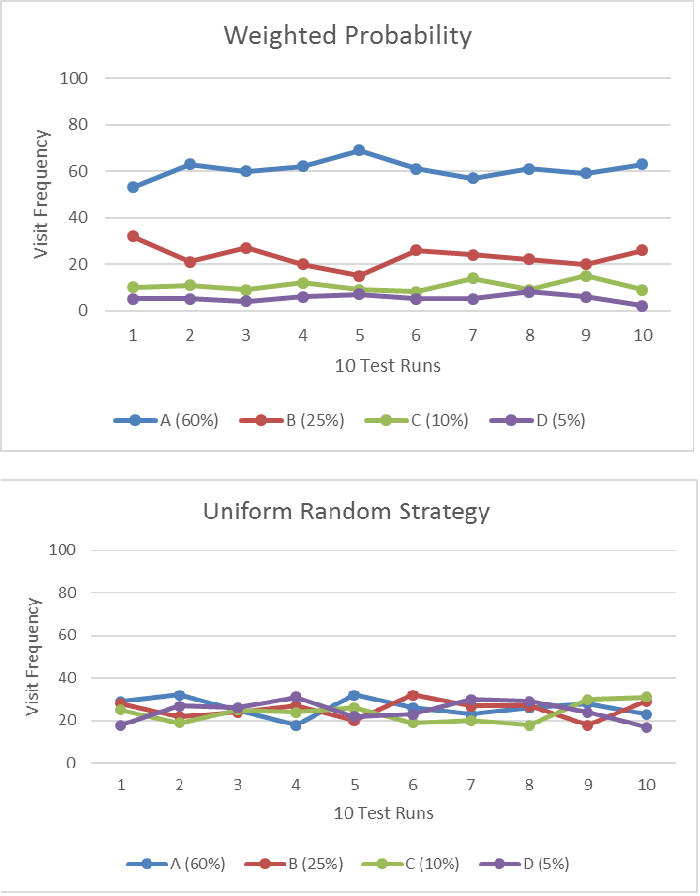
\includegraphics[scale=0.4]{./Images/OCSG_URS_Demo.png}
\caption{A comparison between using weighted probability (above) and uniform probability (below) in selecting patches.}
\end{center}
\end{figure}

The capability of the scheduling program in handling high and low priority areas can be seen in Figure 8. The first chart shows the visit frequencies received by \textit{Area 1}, the patch with the biggest weight value among eight patches. The second shows visit frequencies for Area 8, the lowest priority.

In the first chart, the data shows that the OCSG algorithm is more effecient in deploying patrols to key areas. When given only three patrols, the algorithm deploys patrols to Area 1 at the rate as URS with five patrols. The second chart shows that the algorithm visited Area 8 less than URS, but this is caused by the OCSG algorithm's tendency to visit higher priority areas more often. URS only assigns randomly regardless of the actual patch's susceptibility to threats, and from a security standpoint, this is not considered effective.

\begin{figure}
\begin{center}
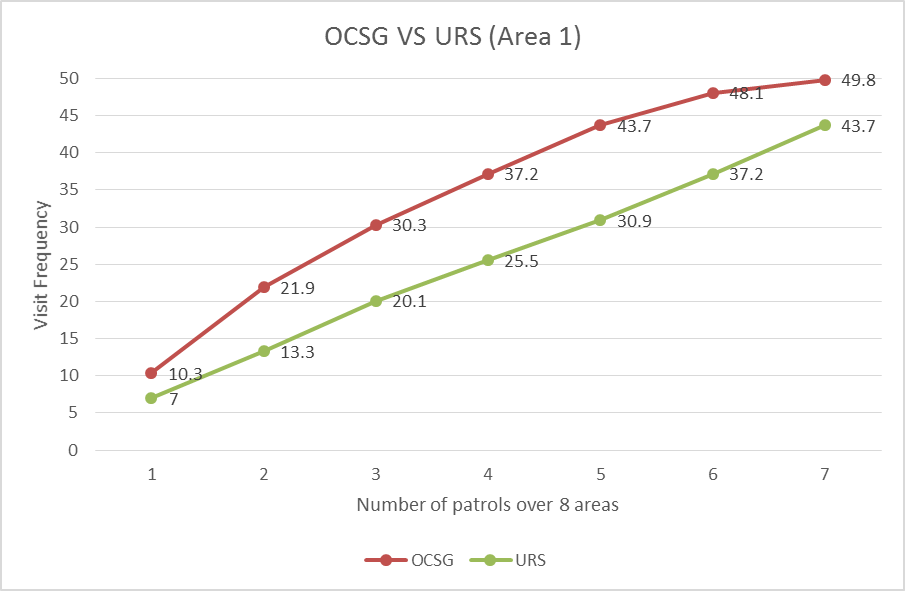
\includegraphics[scale=0.45]{./Images/image027.png}
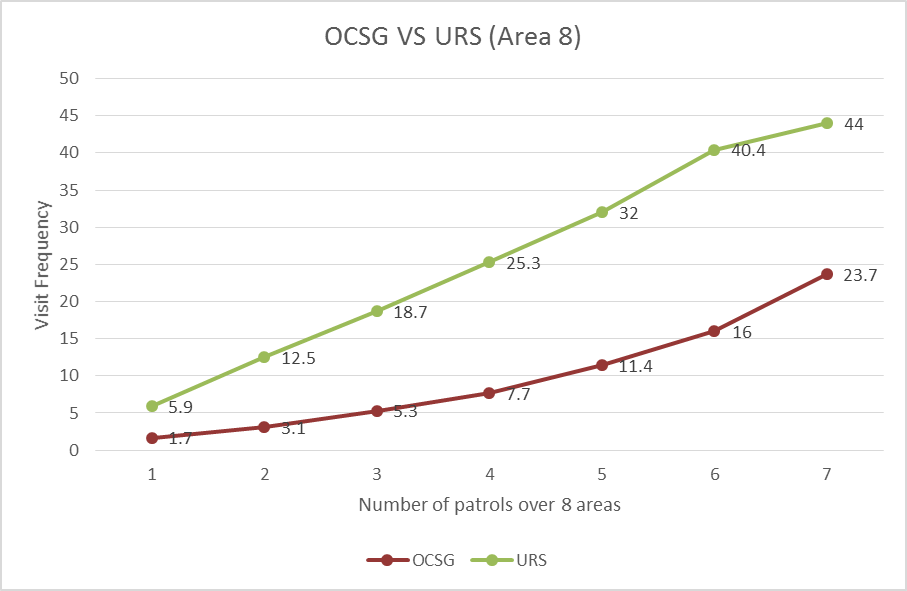
\includegraphics[scale=0.45]{./Images/image029.png}
\caption{The OCSG algorithm deploys patrols more frequently to higher priority patches, without completely neglecting the others.}
\end{center}
\end{figure}

The key to avoiding predictability lies with the randomization of the visit timings. As enemies watch and observe movement, they are able to approximate how often an area is visited, but they will find it difficult to figure out the timings of the patrols. Simply put, they may be able to estimate how often a patrol is deployed in a patch, but they cannot predict when the patrol will be deployed again there. The uncertainty brought about by constantly changing patterns is often enough to discourage them from attempting attacks.

The scheduler does not provide explicit directions to patrols. Patrols are only instructed to relocate to a patch and patrol the surrounding area. This is done in order to provide patrols freedom in their movements. Micro-management of patrols could be discomforting to personnel, as following explicit sets of instructions could take away their sense of freedom.

There are several limitations that this system is facing. Several of those brought upon by the zoning approach. The user cannot transfer a patrol to a different zone, which if enabled could be an opportunity for more flexible schedules. Patrols within a zone still have a tendency to be concentrated in one area of the zone. Problems also arise if a zone does not have at least one patrol in it, because the program would simply leave the zone unattended and vulnerable.

The scheduling procedure has some limitations as well. The algorithm uses the same weight values across its duration, which means that the user has to create a new schedule if the weights are no longer suitable for the situation. The program is also not designed to create schedules that span multiple shifts. If the user would want to schedule a 24-hour day with three shifts, for example, the scheduler would need to be set up and run three separate times.

The algorithm for assigning patrols to patches is somewhat simplistic and primitive. The assignments take into account only the next interval, not the rest of the schedule. There are still possible schedules in which the patrols have significant differences in mileages. If there is a way for the program to look ahead into the schedule when assigning patrols, there is potential for reducing the average mileages further.

When it comes to determining travel distances, it would be better for the program to be given a patrol's real time location data rather than static distance values based on where the patrol is assigned. This would be useful for adjusting the schedule if a patrol had to respond to an emergency situation. In its current state, the program is not capable of receiving and computing real-time location such as data from Global Positioning System (GPS).

% CONCLUSION AND FUTURE WORK
\section{Conclusion and Future Work}
This scheduler is capable of determining optimal strategies for deploying patrols around the UPLB campus. Deployments are effective in making sure that high-priority areas get an adequate amount of visits, while lower priority areas are not left completely vulnerable. Implementing randomization helps in avoiding predictability. Adversaries would find it harder to find attack opportunities as the patrols follow ever changing patterns. Overall, this system can make patrols more effective without increasing the cost.

The current implementation of the program has several limitations. The main targets for improvement would be in the implementations for zoning, scheduling and patrol allocations. A more dynamic approach would enable more dynamic and adaptive solutions. One possible solution for the zoning programs is to dynamically divide the campus according to the number of patrols. The divisions would need to be done within the program, but theoretically this would maximize the spread of patrols, which reduces the response time.

If possible, the simulation should be integrated into the program itself. Having to run the scheduler and the simulation programs separately would mean that data sharing between the two would be prone to errors, human error in particular. If the simulation program is successfully integrated, it could also provide the patrol agents' location data in real-time to the scheduler. Given the said data, the scheduling program can perform more accurate computations, particularly in patrol mileages.

After further refinements, future studies may adapt the scheduling algorithm for use in other areas facing urban crime. There would be distinct differences between domains, but the principle of weighted probabilities and mixed strategies remain the same. Future studies may work on larger, more open domains, such as subdivisions, or in public events and conventions.

\section*{Acknowledgement}
Many thanks to Sir Jade for the patience, guidance, and words of encouragement that allowed me to work and persevere with this study. To my parents, colleagues, and friends, who both knowingly and unknowingly contributed to my research and my well being. And lastly, to the stray cats who let me pet them to calm my mind.


\bibliographystyle{./IEEE/IEEEtran}
\bibliography{./journal}


%%%%%%%%%%%%%%%%%%%%%%%%%%%%%%%%%%%%%%%%%%%%%%%%%%%


% APPENDICES
%\appendices

%\section{Proof of the First Zonklar Equation}
%Appendix one text goes here...

%\section{}
%Appendix two (without title) text goes here...

% ACKNOWLEDGMENT
%\section*{Acknowledgment}
%Many thanks to...

% BIBLIOGRAPHY
%\bibliographystyle{./IEEE/IEEEtran}
%\bibliography{./journal.bib}


% BIOGRAPHY
%\begin{biography}[{\includegraphics{./yourPicture.eps}}]{Student M. Name}
%Biography text here...
%\end{biography}


\end{document}
 
